\documentclass{article}
\usepackage[utf8]{inputenc}
\usepackage{polyglossia}
\usepackage{amssymb,amsmath,amsthm}
\usepackage{bussproofs}
\usepackage{enumitem}
\usepackage{fontspec}
\usepackage{tabularx}
\setdefaultlanguage{russian}
\setotherlanguage{english}
\usepackage{translator}
\uselanguage{russian}
\languagepath{russian}
\setmainfont[Ligatures={TeX,Historic}]{CMU Serif}
\setsansfont{CMU Sans Serif}                    %% задаёт шрифт без засечек
\setmonofont{CMU Typewriter Text}               %% задаёт моноширинный шрифт
\usepackage[a4paper, margin=0.5cm]{geometry}
\usepackage{listings}
\usepackage{graphicx}
\pagenumbering{gobble}
%opening
\title{}
\author{}

\begin{document}

%\maketitle
%https://www.youtube.com/playlist?list=PLlb7e2G7aSpS634rDf15afbmKJRSYmH50

\section*{Измерения SAT-Solver}


\begin{tabularx}{0.8\textwidth} { 
	| >{\raggedright\arraybackslash}X 
	| >{\raggedright\arraybackslash}X 
	| >{\raggedright\arraybackslash}X 
  | >{\raggedright\arraybackslash}X
  | >{\raggedright\arraybackslash}X
	| >{\raggedright\arraybackslash}X  | }
   \hline
   Laptop & CPU & OS & RAM & .NET version  & Configuration\\
   \hline
   HP Victus 16& Ryzen 5 5600H  & Ubuntu 22.10  & 16 GB & 6.0.116 & Release  \\
  \hline
  \end{tabularx}

\subsubsection*{Подготовка к измерениям}
Производительность солвера измерялась на 3-CNF SAT наборе из 100 переменных и 449 дизъюнкта. 
Перед измерениями была зафиксирована частота процессора на 3.3 GHz, 
а также закрыты IDE, браузер, мессенджеры и т.д. 
Поскольку первое измерение заметно больше остальных по времени, солвер сначала "разгоняется", разрешая формулу 5 раз.

\subsubsection*{Сырые данные}
После 40 запусков солвера были получены следующие результаты времени работы:
0.268, 0.26, 0.268, 0.263, 0.262, 0.271, 0.264, 0.263, 0.271, 
0.265, 0.265, 0.272, 0.266, 0.266, 0.271, 0.264, 0.262, 0.268, 
0.264, 0.264, 0.268, 0.265, 0.265, 0.267, 0.263, 0.268, 0.263, 
0.264, 0.266, 0.269, 0.259, 0.264, 0.271, 0.265, 0.266, 0.267, 
0.271, 0.263, 0.265.






\subsubsection*{Гистограмма и p-value}

\begin{figure}[h]
  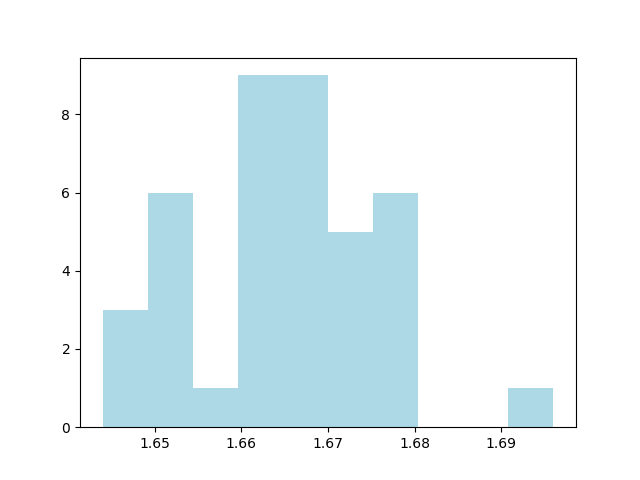
\includegraphics[height=10cm]{Figure_2.png}
\end{figure}

\begin{tabularx}{0.8\textwidth} { 
	| >{\raggedright\arraybackslash}X 
	| >{\raggedright\arraybackslash}X 
	| >{\raggedright\arraybackslash}X 
	| >{\raggedright\arraybackslash}X  | }
   \hline
   Среднее значение & Стандартное отклонение  & Стандартное отклонение среднего & p-value \\
   \hline
      0.266  & 0.003 & 0.0009  & 0.743\\
  \hline
  \end{tabularx}

  \subsubsection*{Доверительный и предсказывающий интервалы}
  \[ \text{ Доверительный интервал: } \overline{x} \pm 2 \cdot \sigma_{msd} \]
  \[ \text { Предсказывающий интервал: } \overline{x} \pm 2 \cdot \sigma_{sd} \]

  \begin{tabularx}{0.8\textwidth} { 
    | >{\raggedright\arraybackslash}X  
    | >{\raggedright\arraybackslash}X  | }
     \hline
     Доверительный интервал & Предсказывающий интервал \\
     \hline
       0.266 \pm 0.0018   & 0.266 \pm 0.006  \\
    \hline
    \end{tabularx}
\end{document}

